% Shared vector grammar. Generated figure TeX files inline this source.
\documentclass[tikz,border=4mm,12pt]{standalone}
\usepackage[UTF8,fontset=fandol]{ctex}
\usepackage{amsmath,amssymb,bm}
\renewcommand{\familydefault}{\sfdefault}
\hyphenpenalty=10000
\exhyphenpenalty=10000
\usetikzlibrary{arrows.meta,backgrounds,calc}
\definecolor{Ink}{HTML}{273648}
\definecolor{Muted}{HTML}{607086}
\definecolor{Ctx}{HTML}{85898F}
\definecolor{Qst}{HTML}{4F8FA5}
\definecolor{Opt}{HTML}{5A9A6E}
\definecolor{Gen}{HTML}{B89A5E}
\definecolor{Hid}{HTML}{8A74B5}
\definecolor{Wgt}{HTML}{E0904F}
\definecolor{Lgt}{HTML}{C95B5B}
\definecolor{Idx}{HTML}{7E8B9B}
\definecolor{Msk}{HTML}{3F5A78}
\newcommand{\Unit}{0.30}
\newcommand{\Offset}{0.12}
\newcommand{\BinarySupport}{0}
\newcounter{texture}
\tikzset{
 flow/.style={-{Latex[length=2mm,width=1.5mm]},draw=Ink!75!Canvas,line width=.65pt},
 tensorlabel/.style={font=\small,text=Ink,align=center,inner sep=0pt},
 tenshape/.style={font=\scriptsize,text=Muted,align=center,inner sep=0pt},
 stage/.style={font=\small\bfseries,text=Muted,align=left,anchor=west},
 operation/.style={draw=Ink!25!Canvas,fill=Canvas,rounded corners=2pt,align=center,
  font=\small,text=Ink,inner sep=5pt,line width=.5pt},
}
% The last two axes define a matrix face. Leading axes use offset sheets.
% Every symbolic dimension maps to the same cell count throughout the set.
\newcommand{\Tensor}[9]{%
 \stepcounter{texture}
 \pgfmathsetmacro{\ww}{#5*\Unit}
 \pgfmathsetmacro{\hh}{#4*\Unit}
 \pgfmathsetmacro{\xx}{#2-\ww/2}
 \pgfmathsetmacro{\yy}{#3-\hh/2}
 \ifnum#7>0
  \foreach \s in {#7,...,1}{
   \path[draw=#6!40!Canvas,fill=Canvas,line width=.45pt,rounded corners=.7pt]
    ({\xx+\s*\Offset},{\yy+\s*\Offset}) rectangle ++(\ww,\hh);}
 \fi
 \foreach \r in {1,...,#4}{\foreach \c in {1,...,#5}{
  \ifnum\BinarySupport>0
   \pgfmathtruncatemacro{\level}{\BinarySupport==1?(\c>3-\r?75:0):(\BinarySupport==2?(\c<=4-\r?75:0):(\c<=\r?75:0))}
  \else
   \pgfmathtruncatemacro{\tone}{mod(\r*13+\c*7+\arabic{texture}*11,7)}
   \pgfmathtruncatemacro{\level}{\tone<3?30:(\tone<6?55:80)}
  \fi
  \path[fill=#6!\level!Canvas,rounded corners=.5pt]
   ({\xx+(\c-1)*\Unit+.021},{\yy+\hh-\r*\Unit+.021})
    rectangle ++({\Unit-.042},{\Unit-.042});}}
 \ifnum\BinarySupport>0
  \path[draw=Msk!35!Canvas,line width=.4pt] (\xx,\yy) rectangle ++(\ww,\hh);
 \fi
 \coordinate (#1-w) at (\xx,#3);
 \coordinate (#1-e) at ({\xx+\ww+#7*\Offset},#3);
 \node[tensorlabel] at (#2,{\yy-.28}) {$#8$};
 \node[tenshape] at (#2,{\yy-.63}) {$#9$};
}
% Exact binary support; row i is a query and column j a key.
\newcommand{\Support}[5]{%
 \foreach \i in {1,...,#4}{\foreach \j in {1,...,#4}{
  \pgfmathtruncatemacro{\on}{#5}
  \ifnum\on>0
   \path[fill=Msk!65!Canvas,rounded corners=.4pt]
    ({#2+(\j-1)*\Unit+.021},{#3-\i*\Unit+.021})
     rectangle ++({\Unit-.042},{\Unit-.042});
  \fi}}
 \path[draw=Ink!35!Canvas,line width=.4pt] (#2,#3) rectangle ++({#4*\Unit},{-#4*\Unit});
}
\newcommand{\Meaning}[7]{%
 \node[anchor=north west,fill=Ink!4!Canvas,rounded corners=3pt,inner sep=9pt,
  text width=#3cm-18pt,align=left,font=\small] (meaning) at (#1,#2) {
  \begin{tabular}{@{}p{1.8cm}@{\hspace{7pt}}p{\dimexpr #3cm-2.8cm\relax}@{}}
   \textbf{#4} & \raggedright #5\tabularnewline[6pt]
   \textbf{#6} & \raggedright #7\tabularnewline
  \end{tabular}};
}

\definecolor{Canvas}{HTML}{18212C}
\definecolor{Ink}{HTML}{E2EAF3}
\definecolor{Muted}{HTML}{AABCD0}
\definecolor{Ctx}{HTML}{ABB3BE}
\definecolor{Qst}{HTML}{72B8D0}
\definecolor{Opt}{HTML}{83C396}
\definecolor{Gen}{HTML}{D9BC7B}
\definecolor{Hid}{HTML}{B49BDB}
\definecolor{Wgt}{HTML}{F0AB71}
\definecolor{Lgt}{HTML}{ED9191}
\definecolor{Idx}{HTML}{A9BBD1}
\definecolor{Msk}{HTML}{91B6DF}
\pagecolor{Canvas}

\providecolor{Canvas}{HTML}{FFFFFF}
\begin{document}
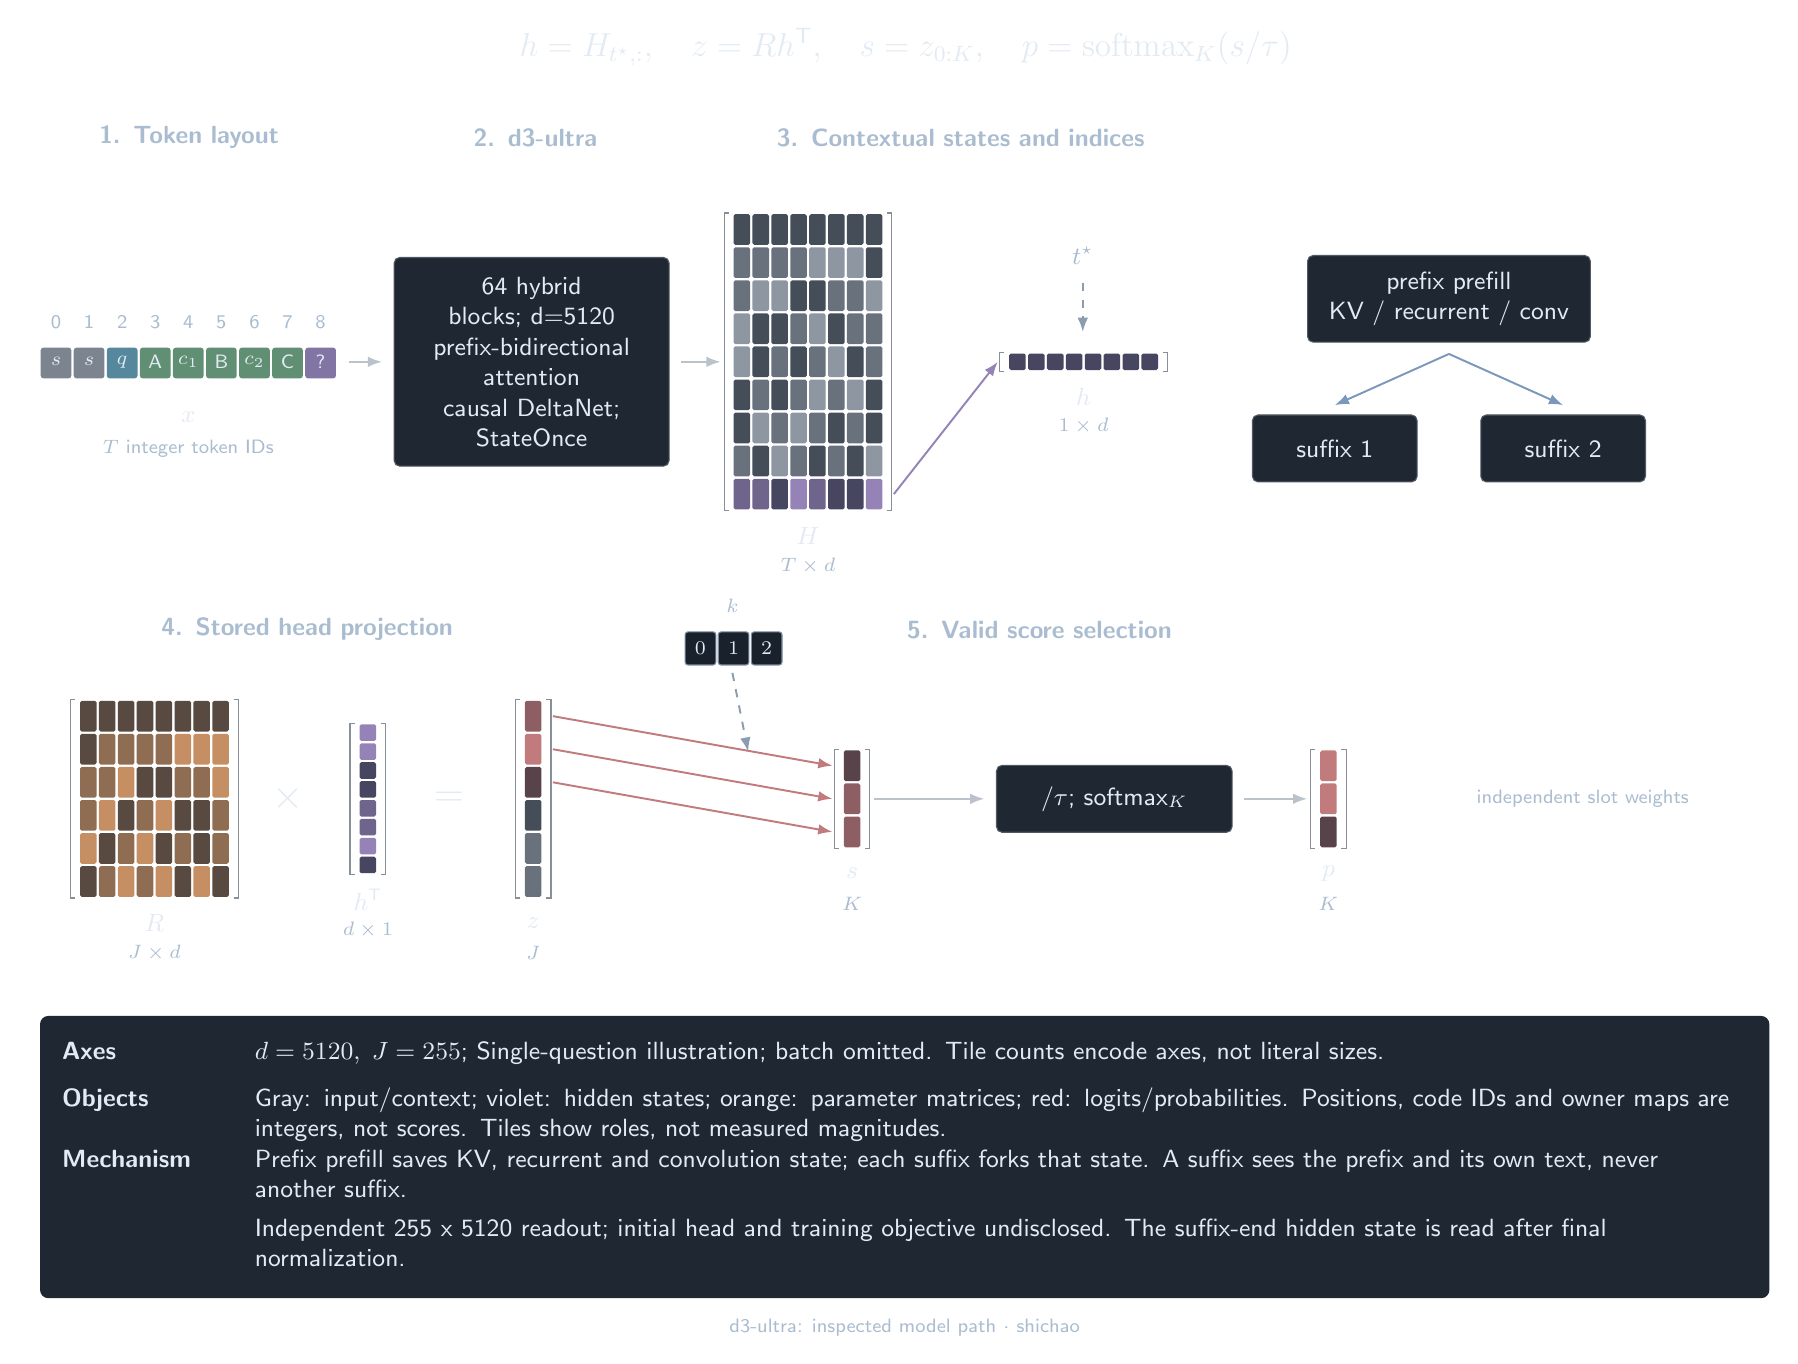
\begin{tikzpicture}[x=1cm,y=1cm,text=Ink]
\node[font=\large,text=Ink,anchor=center,align=center,inner sep=0pt] at (11.000,4.000) {$\displaystyle h=H_{t^\star,:},\quad z=R h^{\mathsf T},\quad s=z_{0:K},\quad p=\operatorname{softmax}_K(s/\tau)$};
\node[font=\small,text=Muted,anchor=center,align=center,inner sep=0pt,text width=4.1cm] at (1.900,2.850) {\textbf{1. Token layout}};
\node[font=\small,text=Muted,anchor=center,align=center,inner sep=0pt,text width=3.6cm] at (6.300,2.850) {\textbf{2. d3-ultra}};
\node[font=\small,text=Muted,anchor=center,align=center,inner sep=0pt,text width=5.6cm] at (11.700,2.850) {\textbf{3. Contextual states and indices}};
\path[fill=Ctx!68!Canvas,rounded corners=1pt] (0.015,-0.210) rectangle ++(0.390,0.390);
\node[font=\scriptsize,text=Ink,anchor=center,align=center,inner sep=0pt] at (0.210,0.000) {$s$};
\node[font=\scriptsize,text=Muted,anchor=center,align=center,inner sep=0pt] at (0.210,0.500) {0};
\path[fill=Ctx!68!Canvas,rounded corners=1pt] (0.435,-0.210) rectangle ++(0.390,0.390);
\node[font=\scriptsize,text=Ink,anchor=center,align=center,inner sep=0pt] at (0.630,0.000) {$s$};
\node[font=\scriptsize,text=Muted,anchor=center,align=center,inner sep=0pt] at (0.630,0.500) {1};
\path[fill=Qst!68!Canvas,rounded corners=1pt] (0.855,-0.210) rectangle ++(0.390,0.390);
\node[font=\scriptsize,text=Ink,anchor=center,align=center,inner sep=0pt] at (1.050,0.000) {$q$};
\node[font=\scriptsize,text=Muted,anchor=center,align=center,inner sep=0pt] at (1.050,0.500) {2};
\path[fill=Opt!68!Canvas,rounded corners=1pt] (1.275,-0.210) rectangle ++(0.390,0.390);
\node[font=\scriptsize,text=Ink,anchor=center,align=center,inner sep=0pt] at (1.470,0.000) {A};
\node[font=\scriptsize,text=Muted,anchor=center,align=center,inner sep=0pt] at (1.470,0.500) {3};
\path[fill=Opt!68!Canvas,rounded corners=1pt] (1.695,-0.210) rectangle ++(0.390,0.390);
\node[font=\scriptsize,text=Ink,anchor=center,align=center,inner sep=0pt] at (1.890,0.000) {$c_1$};
\node[font=\scriptsize,text=Muted,anchor=center,align=center,inner sep=0pt] at (1.890,0.500) {4};
\path[fill=Opt!68!Canvas,rounded corners=1pt] (2.115,-0.210) rectangle ++(0.390,0.390);
\node[font=\scriptsize,text=Ink,anchor=center,align=center,inner sep=0pt] at (2.310,0.000) {B};
\node[font=\scriptsize,text=Muted,anchor=center,align=center,inner sep=0pt] at (2.310,0.500) {5};
\path[fill=Opt!68!Canvas,rounded corners=1pt] (2.535,-0.210) rectangle ++(0.390,0.390);
\node[font=\scriptsize,text=Ink,anchor=center,align=center,inner sep=0pt] at (2.730,0.000) {$c_2$};
\node[font=\scriptsize,text=Muted,anchor=center,align=center,inner sep=0pt] at (2.730,0.500) {6};
\path[fill=Opt!68!Canvas,rounded corners=1pt] (2.955,-0.210) rectangle ++(0.390,0.390);
\node[font=\scriptsize,text=Ink,anchor=center,align=center,inner sep=0pt] at (3.150,0.000) {C};
\node[font=\scriptsize,text=Muted,anchor=center,align=center,inner sep=0pt] at (3.150,0.500) {7};
\path[fill=Hid!68!Canvas,rounded corners=1pt] (3.375,-0.210) rectangle ++(0.390,0.390);
\node[font=\scriptsize,text=Ink,anchor=center,align=center,inner sep=0pt] at (3.570,0.000) {?};
\node[font=\scriptsize,text=Muted,anchor=center,align=center,inner sep=0pt] at (3.570,0.500) {8};
\node[font=\small,text=Ink,anchor=center,align=center,inner sep=0pt] at (1.890,-0.700) {$x$};
\node[font=\scriptsize,text=Muted,anchor=center,align=center,inner sep=0pt] at (1.890,-1.100) {$T$ integer token IDs};
\node[draw=Ink!28!Canvas,fill=Ink!3!Canvas,rounded corners=2pt,font=\small,text width=3.280cm,align=center,inner sep=3pt,minimum height=2.650cm] at (6.250,0.000) {64 hybrid blocks; d=5120\\prefix-bidirectional attention\\causal DeltaNet; StateOnce};
\path[fill=Ctx!30!Canvas,rounded corners=.6pt] (8.815,1.485) rectangle ++(0.210,0.390);
\path[fill=Ctx!30!Canvas,rounded corners=.6pt] (9.055,1.485) rectangle ++(0.210,0.390);
\path[fill=Ctx!30!Canvas,rounded corners=.6pt] (9.295,1.485) rectangle ++(0.210,0.390);
\path[fill=Ctx!30!Canvas,rounded corners=.6pt] (9.535,1.485) rectangle ++(0.210,0.390);
\path[fill=Ctx!30!Canvas,rounded corners=.6pt] (9.775,1.485) rectangle ++(0.210,0.390);
\path[fill=Ctx!30!Canvas,rounded corners=.6pt] (10.015,1.485) rectangle ++(0.210,0.390);
\path[fill=Ctx!30!Canvas,rounded corners=.6pt] (10.255,1.485) rectangle ++(0.210,0.390);
\path[fill=Ctx!30!Canvas,rounded corners=.6pt] (10.495,1.485) rectangle ++(0.210,0.390);
\path[fill=Ctx!55!Canvas,rounded corners=.6pt] (8.815,1.065) rectangle ++(0.210,0.390);
\path[fill=Ctx!55!Canvas,rounded corners=.6pt] (9.055,1.065) rectangle ++(0.210,0.390);
\path[fill=Ctx!55!Canvas,rounded corners=.6pt] (9.295,1.065) rectangle ++(0.210,0.390);
\path[fill=Ctx!55!Canvas,rounded corners=.6pt] (9.535,1.065) rectangle ++(0.210,0.390);
\path[fill=Ctx!80!Canvas,rounded corners=.6pt] (9.775,1.065) rectangle ++(0.210,0.390);
\path[fill=Ctx!80!Canvas,rounded corners=.6pt] (10.015,1.065) rectangle ++(0.210,0.390);
\path[fill=Ctx!80!Canvas,rounded corners=.6pt] (10.255,1.065) rectangle ++(0.210,0.390);
\path[fill=Ctx!30!Canvas,rounded corners=.6pt] (10.495,1.065) rectangle ++(0.210,0.390);
\path[fill=Ctx!55!Canvas,rounded corners=.6pt] (8.815,0.645) rectangle ++(0.210,0.390);
\path[fill=Ctx!80!Canvas,rounded corners=.6pt] (9.055,0.645) rectangle ++(0.210,0.390);
\path[fill=Ctx!80!Canvas,rounded corners=.6pt] (9.295,0.645) rectangle ++(0.210,0.390);
\path[fill=Ctx!30!Canvas,rounded corners=.6pt] (9.535,0.645) rectangle ++(0.210,0.390);
\path[fill=Ctx!30!Canvas,rounded corners=.6pt] (9.775,0.645) rectangle ++(0.210,0.390);
\path[fill=Ctx!55!Canvas,rounded corners=.6pt] (10.015,0.645) rectangle ++(0.210,0.390);
\path[fill=Ctx!55!Canvas,rounded corners=.6pt] (10.255,0.645) rectangle ++(0.210,0.390);
\path[fill=Ctx!80!Canvas,rounded corners=.6pt] (10.495,0.645) rectangle ++(0.210,0.390);
\path[fill=Ctx!80!Canvas,rounded corners=.6pt] (8.815,0.225) rectangle ++(0.210,0.390);
\path[fill=Ctx!30!Canvas,rounded corners=.6pt] (9.055,0.225) rectangle ++(0.210,0.390);
\path[fill=Ctx!30!Canvas,rounded corners=.6pt] (9.295,0.225) rectangle ++(0.210,0.390);
\path[fill=Ctx!55!Canvas,rounded corners=.6pt] (9.535,0.225) rectangle ++(0.210,0.390);
\path[fill=Ctx!80!Canvas,rounded corners=.6pt] (9.775,0.225) rectangle ++(0.210,0.390);
\path[fill=Ctx!30!Canvas,rounded corners=.6pt] (10.015,0.225) rectangle ++(0.210,0.390);
\path[fill=Ctx!55!Canvas,rounded corners=.6pt] (10.255,0.225) rectangle ++(0.210,0.390);
\path[fill=Ctx!55!Canvas,rounded corners=.6pt] (10.495,0.225) rectangle ++(0.210,0.390);
\path[fill=Ctx!80!Canvas,rounded corners=.6pt] (8.815,-0.195) rectangle ++(0.210,0.390);
\path[fill=Ctx!30!Canvas,rounded corners=.6pt] (9.055,-0.195) rectangle ++(0.210,0.390);
\path[fill=Ctx!55!Canvas,rounded corners=.6pt] (9.295,-0.195) rectangle ++(0.210,0.390);
\path[fill=Ctx!30!Canvas,rounded corners=.6pt] (9.535,-0.195) rectangle ++(0.210,0.390);
\path[fill=Ctx!55!Canvas,rounded corners=.6pt] (9.775,-0.195) rectangle ++(0.210,0.390);
\path[fill=Ctx!80!Canvas,rounded corners=.6pt] (10.015,-0.195) rectangle ++(0.210,0.390);
\path[fill=Ctx!30!Canvas,rounded corners=.6pt] (10.255,-0.195) rectangle ++(0.210,0.390);
\path[fill=Ctx!55!Canvas,rounded corners=.6pt] (10.495,-0.195) rectangle ++(0.210,0.390);
\path[fill=Ctx!30!Canvas,rounded corners=.6pt] (8.815,-0.615) rectangle ++(0.210,0.390);
\path[fill=Ctx!55!Canvas,rounded corners=.6pt] (9.055,-0.615) rectangle ++(0.210,0.390);
\path[fill=Ctx!30!Canvas,rounded corners=.6pt] (9.295,-0.615) rectangle ++(0.210,0.390);
\path[fill=Ctx!55!Canvas,rounded corners=.6pt] (9.535,-0.615) rectangle ++(0.210,0.390);
\path[fill=Ctx!80!Canvas,rounded corners=.6pt] (9.775,-0.615) rectangle ++(0.210,0.390);
\path[fill=Ctx!55!Canvas,rounded corners=.6pt] (10.015,-0.615) rectangle ++(0.210,0.390);
\path[fill=Ctx!80!Canvas,rounded corners=.6pt] (10.255,-0.615) rectangle ++(0.210,0.390);
\path[fill=Ctx!30!Canvas,rounded corners=.6pt] (10.495,-0.615) rectangle ++(0.210,0.390);
\path[fill=Ctx!30!Canvas,rounded corners=.6pt] (8.815,-1.035) rectangle ++(0.210,0.390);
\path[fill=Ctx!80!Canvas,rounded corners=.6pt] (9.055,-1.035) rectangle ++(0.210,0.390);
\path[fill=Ctx!55!Canvas,rounded corners=.6pt] (9.295,-1.035) rectangle ++(0.210,0.390);
\path[fill=Ctx!80!Canvas,rounded corners=.6pt] (9.535,-1.035) rectangle ++(0.210,0.390);
\path[fill=Ctx!55!Canvas,rounded corners=.6pt] (9.775,-1.035) rectangle ++(0.210,0.390);
\path[fill=Ctx!30!Canvas,rounded corners=.6pt] (10.015,-1.035) rectangle ++(0.210,0.390);
\path[fill=Ctx!55!Canvas,rounded corners=.6pt] (10.255,-1.035) rectangle ++(0.210,0.390);
\path[fill=Ctx!30!Canvas,rounded corners=.6pt] (10.495,-1.035) rectangle ++(0.210,0.390);
\path[fill=Ctx!55!Canvas,rounded corners=.6pt] (8.815,-1.455) rectangle ++(0.210,0.390);
\path[fill=Ctx!30!Canvas,rounded corners=.6pt] (9.055,-1.455) rectangle ++(0.210,0.390);
\path[fill=Ctx!80!Canvas,rounded corners=.6pt] (9.295,-1.455) rectangle ++(0.210,0.390);
\path[fill=Ctx!55!Canvas,rounded corners=.6pt] (9.535,-1.455) rectangle ++(0.210,0.390);
\path[fill=Ctx!30!Canvas,rounded corners=.6pt] (9.775,-1.455) rectangle ++(0.210,0.390);
\path[fill=Ctx!55!Canvas,rounded corners=.6pt] (10.015,-1.455) rectangle ++(0.210,0.390);
\path[fill=Ctx!30!Canvas,rounded corners=.6pt] (10.255,-1.455) rectangle ++(0.210,0.390);
\path[fill=Ctx!80!Canvas,rounded corners=.6pt] (10.495,-1.455) rectangle ++(0.210,0.390);
\path[fill=Hid!55!Canvas,rounded corners=.6pt] (8.815,-1.875) rectangle ++(0.210,0.390);
\path[fill=Hid!55!Canvas,rounded corners=.6pt] (9.055,-1.875) rectangle ++(0.210,0.390);
\path[fill=Hid!30!Canvas,rounded corners=.6pt] (9.295,-1.875) rectangle ++(0.210,0.390);
\path[fill=Hid!80!Canvas,rounded corners=.6pt] (9.535,-1.875) rectangle ++(0.210,0.390);
\path[fill=Hid!55!Canvas,rounded corners=.6pt] (9.775,-1.875) rectangle ++(0.210,0.390);
\path[fill=Hid!30!Canvas,rounded corners=.6pt] (10.015,-1.875) rectangle ++(0.210,0.390);
\path[fill=Hid!30!Canvas,rounded corners=.6pt] (10.255,-1.875) rectangle ++(0.210,0.390);
\path[fill=Hid!80!Canvas,rounded corners=.6pt] (10.495,-1.875) rectangle ++(0.210,0.390);
\draw[draw=Ink!55!Canvas,line width=.45pt] (8.755,1.890) -- ++(-.06,0) -- ++(0,-3.780) -- ++(.06,0);
\draw[draw=Ink!55!Canvas,line width=.45pt] (10.765,1.890) -- ++(.06,0) -- ++(0,-3.780) -- ++(-.06,0);
\node[font=\small,text=Ink,anchor=center,align=center,inner sep=0pt] at (9.760,-2.210) {$H$};
\node[font=\scriptsize,text=Muted,anchor=center,align=center,inner sep=0pt] at (9.760,-2.590) {$T\times d$};
\begin{scope}[on background layer]
\draw[-{Latex[length=1.8mm]},draw=Ink!80!Canvas,line width=.7pt] (3.930,0.000) -- (4.350,0.000);
\end{scope}
\begin{scope}[on background layer]
\draw[-{Latex[length=1.8mm]},draw=Ink!80!Canvas,line width=.7pt] (8.150,0.000) -- (8.650,0.000);
\end{scope}
\path[fill=Hid!30!Canvas,rounded corners=.6pt] (12.315,-0.105) rectangle ++(0.210,0.210);
\path[fill=Hid!30!Canvas,rounded corners=.6pt] (12.555,-0.105) rectangle ++(0.210,0.210);
\path[fill=Hid!30!Canvas,rounded corners=.6pt] (12.795,-0.105) rectangle ++(0.210,0.210);
\path[fill=Hid!30!Canvas,rounded corners=.6pt] (13.035,-0.105) rectangle ++(0.210,0.210);
\path[fill=Hid!30!Canvas,rounded corners=.6pt] (13.275,-0.105) rectangle ++(0.210,0.210);
\path[fill=Hid!30!Canvas,rounded corners=.6pt] (13.515,-0.105) rectangle ++(0.210,0.210);
\path[fill=Hid!30!Canvas,rounded corners=.6pt] (13.755,-0.105) rectangle ++(0.210,0.210);
\path[fill=Hid!30!Canvas,rounded corners=.6pt] (13.995,-0.105) rectangle ++(0.210,0.210);
\draw[draw=Ink!55!Canvas,line width=.45pt] (12.255,0.120) -- ++(-.06,0) -- ++(0,-0.240) -- ++(.06,0);
\draw[draw=Ink!55!Canvas,line width=.45pt] (14.265,0.120) -- ++(.06,0) -- ++(0,-0.240) -- ++(-.06,0);
\node[font=\small,text=Ink,anchor=center,align=center,inner sep=0pt] at (13.260,-0.440) {$h$};
\node[font=\scriptsize,text=Muted,anchor=center,align=center,inner sep=0pt] at (13.260,-0.820) {$1\times d$};
\begin{scope}[on background layer]
\draw[-{Latex[length=1.8mm]},draw=Hid!80!Canvas,line width=.7pt] (10.850,-1.680) -- (12.170,0.000);
\end{scope}
\node[font=\small,text=Idx,anchor=center,align=center,inner sep=0pt] at (13.250,1.350) {$t^\star$};
\begin{scope}[on background layer]
\draw[-{Latex[length=1.8mm]},draw=Idx!80!Canvas,line width=.7pt,dashed] (13.250,1.000) -- (13.250,0.380);
\end{scope}
\node[draw=Ink!28!Canvas,fill=Ink!3!Canvas,rounded corners=2pt,font=\small,text width=3.380cm,align=center,inner sep=3pt,minimum height=1.100cm] at (17.900,0.800) {prefix prefill\\KV / recurrent / conv};
\node[draw=Ink!28!Canvas,fill=Ink!3!Canvas,rounded corners=2pt,font=\small,text width=1.880cm,align=center,inner sep=3pt,minimum height=0.850cm] at (16.450,-1.100) {suffix 1};
\node[draw=Ink!28!Canvas,fill=Ink!3!Canvas,rounded corners=2pt,font=\small,text width=1.880cm,align=center,inner sep=3pt,minimum height=0.850cm] at (19.350,-1.100) {suffix 2};
\begin{scope}[on background layer]
\draw[-{Latex[length=1.8mm]},draw=Msk!80!Canvas,line width=.7pt] (17.900,0.100) -- (16.450,-0.550);
\end{scope}
\begin{scope}[on background layer]
\draw[-{Latex[length=1.8mm]},draw=Msk!80!Canvas,line width=.7pt] (17.900,0.100) -- (19.350,-0.550);
\end{scope}
\node[font=\small,text=Muted,anchor=center,align=center,inner sep=0pt,text width=6cm] at (3.400,-3.400) {\textbf{4. Stored head projection}};
\node[font=\small,text=Muted,anchor=center,align=center,inner sep=0pt,text width=4.8cm] at (12.700,-3.400) {\textbf{5. Valid score selection}};
\path[fill=Wgt!30!Canvas,rounded corners=.6pt] (0.515,-4.695) rectangle ++(0.210,0.390);
\path[fill=Wgt!30!Canvas,rounded corners=.6pt] (0.755,-4.695) rectangle ++(0.210,0.390);
\path[fill=Wgt!30!Canvas,rounded corners=.6pt] (0.995,-4.695) rectangle ++(0.210,0.390);
\path[fill=Wgt!30!Canvas,rounded corners=.6pt] (1.235,-4.695) rectangle ++(0.210,0.390);
\path[fill=Wgt!30!Canvas,rounded corners=.6pt] (1.475,-4.695) rectangle ++(0.210,0.390);
\path[fill=Wgt!30!Canvas,rounded corners=.6pt] (1.715,-4.695) rectangle ++(0.210,0.390);
\path[fill=Wgt!30!Canvas,rounded corners=.6pt] (1.955,-4.695) rectangle ++(0.210,0.390);
\path[fill=Wgt!30!Canvas,rounded corners=.6pt] (2.195,-4.695) rectangle ++(0.210,0.390);
\path[fill=Wgt!30!Canvas,rounded corners=.6pt] (0.515,-5.115) rectangle ++(0.210,0.390);
\path[fill=Wgt!55!Canvas,rounded corners=.6pt] (0.755,-5.115) rectangle ++(0.210,0.390);
\path[fill=Wgt!55!Canvas,rounded corners=.6pt] (0.995,-5.115) rectangle ++(0.210,0.390);
\path[fill=Wgt!55!Canvas,rounded corners=.6pt] (1.235,-5.115) rectangle ++(0.210,0.390);
\path[fill=Wgt!55!Canvas,rounded corners=.6pt] (1.475,-5.115) rectangle ++(0.210,0.390);
\path[fill=Wgt!80!Canvas,rounded corners=.6pt] (1.715,-5.115) rectangle ++(0.210,0.390);
\path[fill=Wgt!80!Canvas,rounded corners=.6pt] (1.955,-5.115) rectangle ++(0.210,0.390);
\path[fill=Wgt!80!Canvas,rounded corners=.6pt] (2.195,-5.115) rectangle ++(0.210,0.390);
\path[fill=Wgt!55!Canvas,rounded corners=.6pt] (0.515,-5.535) rectangle ++(0.210,0.390);
\path[fill=Wgt!55!Canvas,rounded corners=.6pt] (0.755,-5.535) rectangle ++(0.210,0.390);
\path[fill=Wgt!80!Canvas,rounded corners=.6pt] (0.995,-5.535) rectangle ++(0.210,0.390);
\path[fill=Wgt!30!Canvas,rounded corners=.6pt] (1.235,-5.535) rectangle ++(0.210,0.390);
\path[fill=Wgt!30!Canvas,rounded corners=.6pt] (1.475,-5.535) rectangle ++(0.210,0.390);
\path[fill=Wgt!55!Canvas,rounded corners=.6pt] (1.715,-5.535) rectangle ++(0.210,0.390);
\path[fill=Wgt!55!Canvas,rounded corners=.6pt] (1.955,-5.535) rectangle ++(0.210,0.390);
\path[fill=Wgt!80!Canvas,rounded corners=.6pt] (2.195,-5.535) rectangle ++(0.210,0.390);
\path[fill=Wgt!55!Canvas,rounded corners=.6pt] (0.515,-5.955) rectangle ++(0.210,0.390);
\path[fill=Wgt!80!Canvas,rounded corners=.6pt] (0.755,-5.955) rectangle ++(0.210,0.390);
\path[fill=Wgt!30!Canvas,rounded corners=.6pt] (0.995,-5.955) rectangle ++(0.210,0.390);
\path[fill=Wgt!55!Canvas,rounded corners=.6pt] (1.235,-5.955) rectangle ++(0.210,0.390);
\path[fill=Wgt!80!Canvas,rounded corners=.6pt] (1.475,-5.955) rectangle ++(0.210,0.390);
\path[fill=Wgt!30!Canvas,rounded corners=.6pt] (1.715,-5.955) rectangle ++(0.210,0.390);
\path[fill=Wgt!30!Canvas,rounded corners=.6pt] (1.955,-5.955) rectangle ++(0.210,0.390);
\path[fill=Wgt!55!Canvas,rounded corners=.6pt] (2.195,-5.955) rectangle ++(0.210,0.390);
\path[fill=Wgt!80!Canvas,rounded corners=.6pt] (0.515,-6.375) rectangle ++(0.210,0.390);
\path[fill=Wgt!30!Canvas,rounded corners=.6pt] (0.755,-6.375) rectangle ++(0.210,0.390);
\path[fill=Wgt!55!Canvas,rounded corners=.6pt] (0.995,-6.375) rectangle ++(0.210,0.390);
\path[fill=Wgt!80!Canvas,rounded corners=.6pt] (1.235,-6.375) rectangle ++(0.210,0.390);
\path[fill=Wgt!30!Canvas,rounded corners=.6pt] (1.475,-6.375) rectangle ++(0.210,0.390);
\path[fill=Wgt!55!Canvas,rounded corners=.6pt] (1.715,-6.375) rectangle ++(0.210,0.390);
\path[fill=Wgt!30!Canvas,rounded corners=.6pt] (1.955,-6.375) rectangle ++(0.210,0.390);
\path[fill=Wgt!55!Canvas,rounded corners=.6pt] (2.195,-6.375) rectangle ++(0.210,0.390);
\path[fill=Wgt!30!Canvas,rounded corners=.6pt] (0.515,-6.795) rectangle ++(0.210,0.390);
\path[fill=Wgt!55!Canvas,rounded corners=.6pt] (0.755,-6.795) rectangle ++(0.210,0.390);
\path[fill=Wgt!80!Canvas,rounded corners=.6pt] (0.995,-6.795) rectangle ++(0.210,0.390);
\path[fill=Wgt!55!Canvas,rounded corners=.6pt] (1.235,-6.795) rectangle ++(0.210,0.390);
\path[fill=Wgt!80!Canvas,rounded corners=.6pt] (1.475,-6.795) rectangle ++(0.210,0.390);
\path[fill=Wgt!30!Canvas,rounded corners=.6pt] (1.715,-6.795) rectangle ++(0.210,0.390);
\path[fill=Wgt!80!Canvas,rounded corners=.6pt] (1.955,-6.795) rectangle ++(0.210,0.390);
\path[fill=Wgt!30!Canvas,rounded corners=.6pt] (2.195,-6.795) rectangle ++(0.210,0.390);
\draw[draw=Ink!55!Canvas,line width=.45pt] (0.455,-4.290) -- ++(-.06,0) -- ++(0,-2.520) -- ++(.06,0);
\draw[draw=Ink!55!Canvas,line width=.45pt] (2.465,-4.290) -- ++(.06,0) -- ++(0,-2.520) -- ++(-.06,0);
\node[font=\small,text=Ink,anchor=center,align=center,inner sep=0pt] at (1.460,-7.130) {$R$};
\node[font=\scriptsize,text=Muted,anchor=center,align=center,inner sep=0pt] at (1.460,-7.510) {$J\times d$};
\node[font=\Large,text=Ink,anchor=center,align=center,inner sep=0pt] at (3.150,-5.550) {$\times$};
\path[fill=Hid!80!Canvas,rounded corners=.6pt] (4.065,-4.815) rectangle ++(0.210,0.210);
\path[fill=Hid!80!Canvas,rounded corners=.6pt] (4.065,-5.055) rectangle ++(0.210,0.210);
\path[fill=Hid!30!Canvas,rounded corners=.6pt] (4.065,-5.295) rectangle ++(0.210,0.210);
\path[fill=Hid!30!Canvas,rounded corners=.6pt] (4.065,-5.535) rectangle ++(0.210,0.210);
\path[fill=Hid!55!Canvas,rounded corners=.6pt] (4.065,-5.775) rectangle ++(0.210,0.210);
\path[fill=Hid!55!Canvas,rounded corners=.6pt] (4.065,-6.015) rectangle ++(0.210,0.210);
\path[fill=Hid!80!Canvas,rounded corners=.6pt] (4.065,-6.255) rectangle ++(0.210,0.210);
\path[fill=Hid!30!Canvas,rounded corners=.6pt] (4.065,-6.495) rectangle ++(0.210,0.210);
\draw[draw=Ink!55!Canvas,line width=.45pt] (4.005,-4.590) -- ++(-.06,0) -- ++(0,-1.920) -- ++(.06,0);
\draw[draw=Ink!55!Canvas,line width=.45pt] (4.335,-4.590) -- ++(.06,0) -- ++(0,-1.920) -- ++(-.06,0);
\node[font=\small,text=Ink,anchor=center,align=center,inner sep=0pt] at (4.170,-6.830) {$h^{\mathsf T}$};
\node[font=\scriptsize,text=Muted,anchor=center,align=center,inner sep=0pt] at (4.170,-7.210) {$d\times1$};
\node[font=\Large,text=Ink,anchor=center,align=center,inner sep=0pt] at (5.200,-5.550) {$=$};
\path[fill=Lgt!55!Canvas,rounded corners=.6pt] (6.165,-4.695) rectangle ++(0.210,0.390);
\path[fill=Lgt!80!Canvas,rounded corners=.6pt] (6.165,-5.115) rectangle ++(0.210,0.390);
\path[fill=Lgt!30!Canvas,rounded corners=.6pt] (6.165,-5.535) rectangle ++(0.210,0.390);
\path[fill=Ctx!30!Canvas,rounded corners=.6pt] (6.165,-5.955) rectangle ++(0.210,0.390);
\path[fill=Ctx!55!Canvas,rounded corners=.6pt] (6.165,-6.375) rectangle ++(0.210,0.390);
\path[fill=Ctx!55!Canvas,rounded corners=.6pt] (6.165,-6.795) rectangle ++(0.210,0.390);
\draw[draw=Ink!55!Canvas,line width=.45pt] (6.105,-4.290) -- ++(-.06,0) -- ++(0,-2.520) -- ++(.06,0);
\draw[draw=Ink!55!Canvas,line width=.45pt] (6.435,-4.290) -- ++(.06,0) -- ++(0,-2.520) -- ++(-.06,0);
\node[font=\small,text=Ink,anchor=center,align=center,inner sep=0pt] at (6.270,-7.130) {$z$};
\node[font=\scriptsize,text=Muted,anchor=center,align=center,inner sep=0pt] at (6.270,-7.510) {$J$};
\path[fill=Lgt!30!Canvas,rounded corners=.6pt] (10.215,-5.325) rectangle ++(0.210,0.390);
\path[fill=Lgt!55!Canvas,rounded corners=.6pt] (10.215,-5.745) rectangle ++(0.210,0.390);
\path[fill=Lgt!55!Canvas,rounded corners=.6pt] (10.215,-6.165) rectangle ++(0.210,0.390);
\draw[draw=Ink!55!Canvas,line width=.45pt] (10.155,-4.920) -- ++(-.06,0) -- ++(0,-1.260) -- ++(.06,0);
\draw[draw=Ink!55!Canvas,line width=.45pt] (10.485,-4.920) -- ++(.06,0) -- ++(0,-1.260) -- ++(-.06,0);
\node[font=\small,text=Ink,anchor=center,align=center,inner sep=0pt] at (10.320,-6.500) {$s$};
\node[font=\scriptsize,text=Muted,anchor=center,align=center,inner sep=0pt] at (10.320,-6.880) {$K$};
\begin{scope}[on background layer]
\draw[-{Latex[length=1.8mm]},draw=Lgt!80!Canvas,line width=.7pt] (6.520,-4.500) -- (10.070,-5.130);
\end{scope}
\begin{scope}[on background layer]
\draw[-{Latex[length=1.8mm]},draw=Lgt!80!Canvas,line width=.7pt] (6.520,-4.920) -- (10.070,-5.550);
\end{scope}
\begin{scope}[on background layer]
\draw[-{Latex[length=1.8mm]},draw=Lgt!80!Canvas,line width=.7pt] (6.520,-5.340) -- (10.070,-5.970);
\end{scope}
\path[draw=Idx!70!Canvas,fill=Canvas,rounded corners=1pt] (8.200,-3.850) rectangle ++(.39,.42);
\node[font=\scriptsize,text=Ink,anchor=center,align=center,inner sep=0pt] at (8.395,-3.640) {$0$};
\path[draw=Idx!70!Canvas,fill=Canvas,rounded corners=1pt] (8.620,-3.850) rectangle ++(.39,.42);
\node[font=\scriptsize,text=Ink,anchor=center,align=center,inner sep=0pt] at (8.815,-3.640) {$1$};
\path[draw=Idx!70!Canvas,fill=Canvas,rounded corners=1pt] (9.040,-3.850) rectangle ++(.39,.42);
\node[font=\scriptsize,text=Ink,anchor=center,align=center,inner sep=0pt] at (9.235,-3.640) {$2$};
\node[font=\scriptsize,text=Muted,anchor=center,align=center,inner sep=0pt] at (8.800,-3.100) {$k$};
\begin{scope}[on background layer]
\draw[-{Latex[length=1.8mm]},draw=Idx!80!Canvas,line width=.7pt,dashed] (8.800,-3.950) -- (9.000,-4.950);
\end{scope}
\node[draw=Ink!28!Canvas,fill=Ink!3!Canvas,rounded corners=2pt,font=\small,text width=2.780cm,align=center,inner sep=3pt,minimum height=0.850cm] at (13.650,-5.550) {$/\tau$; softmax$_K$};
\begin{scope}[on background layer]
\draw[-{Latex[length=1.8mm]},draw=Ink!80!Canvas,line width=.7pt] (10.600,-5.550) -- (12.000,-5.550);
\end{scope}
\begin{scope}[on background layer]
\draw[-{Latex[length=1.8mm]},draw=Ink!80!Canvas,line width=.7pt] (15.300,-5.550) -- (16.100,-5.550);
\end{scope}
\path[fill=Lgt!80!Canvas,rounded corners=.6pt] (16.265,-5.325) rectangle ++(0.210,0.390);
\path[fill=Lgt!80!Canvas,rounded corners=.6pt] (16.265,-5.745) rectangle ++(0.210,0.390);
\path[fill=Lgt!30!Canvas,rounded corners=.6pt] (16.265,-6.165) rectangle ++(0.210,0.390);
\draw[draw=Ink!55!Canvas,line width=.45pt] (16.205,-4.920) -- ++(-.06,0) -- ++(0,-1.260) -- ++(.06,0);
\draw[draw=Ink!55!Canvas,line width=.45pt] (16.535,-4.920) -- ++(.06,0) -- ++(0,-1.260) -- ++(-.06,0);
\node[font=\small,text=Ink,anchor=center,align=center,inner sep=0pt] at (16.370,-6.500) {$p$};
\node[font=\scriptsize,text=Muted,anchor=center,align=center,inner sep=0pt] at (16.370,-6.880) {$K$};
\node[font=\scriptsize,text=Muted,anchor=center,align=center,inner sep=0pt,text width=3.7cm] at (19.600,-5.550) {independent slot weights};
\node[anchor=north west,fill=Ink!3!Canvas,rounded corners=3pt,inner sep=8pt,font=\small,text width=21.400cm,align=left] (platefooter) at (0,-8.300) {\begin{tabular}{@{}p{2.2cm}@{\hspace{7pt}}p{18.8cm}@{}}\textbf{Axes} & \raggedright $d=5120,\;J=255$; Single-question illustration; batch omitted. Tile counts encode axes, not literal sizes.\tabularnewline[6pt]\textbf{Objects} & \raggedright Gray: input/context; violet: hidden states; orange: parameter matrices; red: logits/probabilities. Positions, code IDs and owner maps are integers, not scores. Tiles show roles, not measured magnitudes.\tabularnewline[6pt]\textbf{Mechanism} & \raggedright Prefix prefill saves KV, recurrent and convolution state; each suffix forks that state. A suffix sees the prefix and its own text, never another suffix.\\[3pt] Independent 255 x 5120 readout; initial head and training objective undisclosed. The suffix-end hidden state is read after final normalization.\tabularnewline\end{tabular}};
\node[font=\scriptsize,text=Muted,anchor=north,inner sep=0pt] at ($(platefooter.south)+(0,-.25)$) {d3-ultra: inspected model path $\cdot$ shichao};
\end{tikzpicture}
\end{document}
